\section{Příklad 2}
% Jako parametr zadejte skupinu (A-H)
\druhyZadani{G}

\subsection{Řešení}

Cílem úkolu je vypočítat napětí a proud rezistoru $R_5$ za využití Théveninovy věty. Théveninova věta říká, 
že můžeme celý obvod zde sestávající ze zdroje stejnosměrného napětí a rezistorů nahradit jedním zdrojem
napětí $U_e$ s vnitřním odporem $R_e$. Tyto hodnoty musíme nyní vypočítat. 

Uzly, na které je připojen rezistor $R_5$ si označíme písmeny $A$ a $B$.

\begin{figure}[H]
\includegraphics[scale=0.5]{Pr2/step1.png}
\centering
\caption{Označení uzlů $A$ a $B$}
\end{figure}

V prvním kroku spočítáme velikost odporu $R_e$. To provedeme tak, že v části obvodu připojené k uzlům $A$ a $B$ nahradíme všechny zdroje napětí spojením nakrátko, a spočítáme ekvivalentní odpor mezi uzly. Po překreslení zjistíme, že jde o kombinaci sériově a paralelně zapojených rezistorů, jejichž celkový odpor vypočítáme následovně:

$$ R_e = \frac{R4(R_3 + R_1 + R_2)}{R_4 + R_3 + R_1 + R_2} \doteq 156,1765 \Omega $$

\begin{figure}[H]
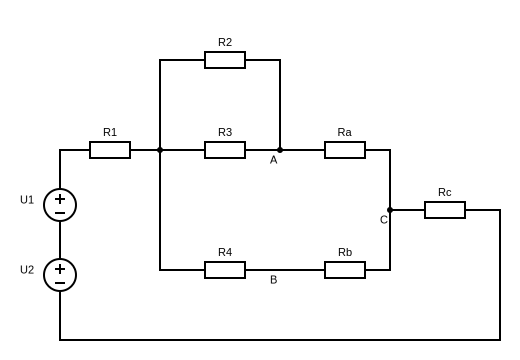
\includegraphics[scale=0.5]{Pr2/step2.png}
\centering
\caption{Překreslené zapojení rezistorů mezi uzly $A$ a $B$}
\end{figure}

Následně vypočteme velikost napětí $U_e$. Napětí $U_e$ je rovno napětí mezi uzly $A$ a $B$, pokud bychom rezistor $R_5$ z obvodu odpojili. V takovém případě nám vznikne zapojení děliče napětí, ve kterém dokážeme napětí mezi uzly $A$ a $B$ snadno vyjádřit jako:

$$ U_e = U \frac{R_4}{R_1 + R_2 + R_3 + R_4} \doteq 23,8235 V $$ 

\begin{figure}[H]
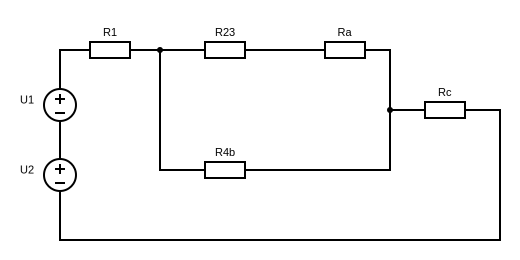
\includegraphics[scale=0.5]{Pr2/step3.png}
\centering
\caption{Původní obvod bez rezistoru $R_5$}
\end{figure}

Nyní můžeme pomocí hodnot $U_e$ a $R_e$ obvod zjednodušit, a dopočítat velikost napětí a proudu na rezistoru $R_5$. Po zakreslení zjednodušeného obvodu si můžeme všimnout, že dostáváme další zapojení děliče napětí, proto můžeme velikost napětí na rezistoru $R_5$ vyjádřit jako:

$$ U_{R5} = U_e \frac{R_5}{R_e + R_5} \doteq 17,7852 V $$

\begin{figure}[H]
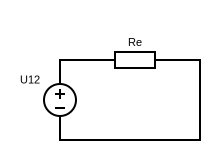
\includegraphics[scale=0.5]{Pr2/final.png}
\centering
\caption{Zjednodušený obvod}
\end{figure}

Velikost proudu pak dopočítáme z Ohmova zákona:

$$ I_{R5} = \frac{U_{R5}}{R_5} \doteq 0,03866 A $$
